\documentclass[12pt]{article}
\usepackage[utf8]{inputenc}
\usepackage[T1]{fontenc}
\usepackage[french]{babel}
\usepackage{graphicx}
\usepackage[top=3cm,bottom=2.5cm,left=2cm,right=2cm]{geometry}

\renewcommand{\contentsname}{Sommaire}
\renewcommand{\thesection}{\Roman{section}-}
\renewcommand{\thesubsection}{\Alph{subsection})}

\newcommand{\Octave}{GNU Octave }
\newcommand{\Matlab}{MATLAB\textsuperscript{\textregistered} }

\title{License SPI -- Projet Auralisation}
\author{Thomas \textsc{Lechat} \and Xin \textsc{Wang} \and Mathieu \textsc{Gaborit}}
\date{Note de synthèse 3 -- Novembre 2012}
\begin{document} \maketitle

\tableofcontents

\section{Rendu perceptif des résultats de la séance précédente} % {{{1

A la séance précédente, une mesure de la réponse impulsionnelle de la salle réverbérante avait été effectuée. Nous avons donc convolué un bruit de claquement de mains trouvé sur Freesound avec la réponse impulsionnelle et avons comparé le rendu à notre propre claquement de mains dans la salle réverbérante. 

D'un point de vu percetif, le résultat est tout à fait satisfaisant une fois débarassé du problème de saturation évoqué ci-après.

\section{Problèmes de convolution sous \Octave/\Matlab} % {{{1

Lors des premiers essais de convolution sous \Octave d'abord et \Matlab ensuite, nous avons noté que les signaux finaux saturaient.

Après plusieurs essais infructueux pour éliminer cette saturation, nous y sommes parvenu en divisant les signaux avant convolution et même après. En effet, c'est la transcription \Matlab $\rightarrow$ WAV qui posait problème (probablement pour des raison de saturation du format WAV).

\section{Script \Matlab} % {{{1

Afin de rendre plus simple le traitement des mesures (et notamment des fichiers textes générés pas \textit{Analyseur CTTM}), nous avons réalisé un script \Matlab/\Octave permettant de récupérer facilement les données.

Il est présent du le dépot du projet et s'utilise comme suit (le second argument étant le nombre de colonnes) :

\begin{verbatim}
data = CTTM_read_txt('nom du fichier', 3)
\end{verbatim}

\section{Enregistrement de l'éclatement d'un ballon en salle anéchoïque} % {{{1

En deuxième partie de séance, un enregistrement de l'éclatement d'un ballon dans la salle anéchoïque est réalisé. Le but de la mesure est de déterminer à quel point la bande passante du ballon avait influé sur les mesures de réponse impulsionnelle de la salle.

\begin{figure}[h!]
	\begin{center}
	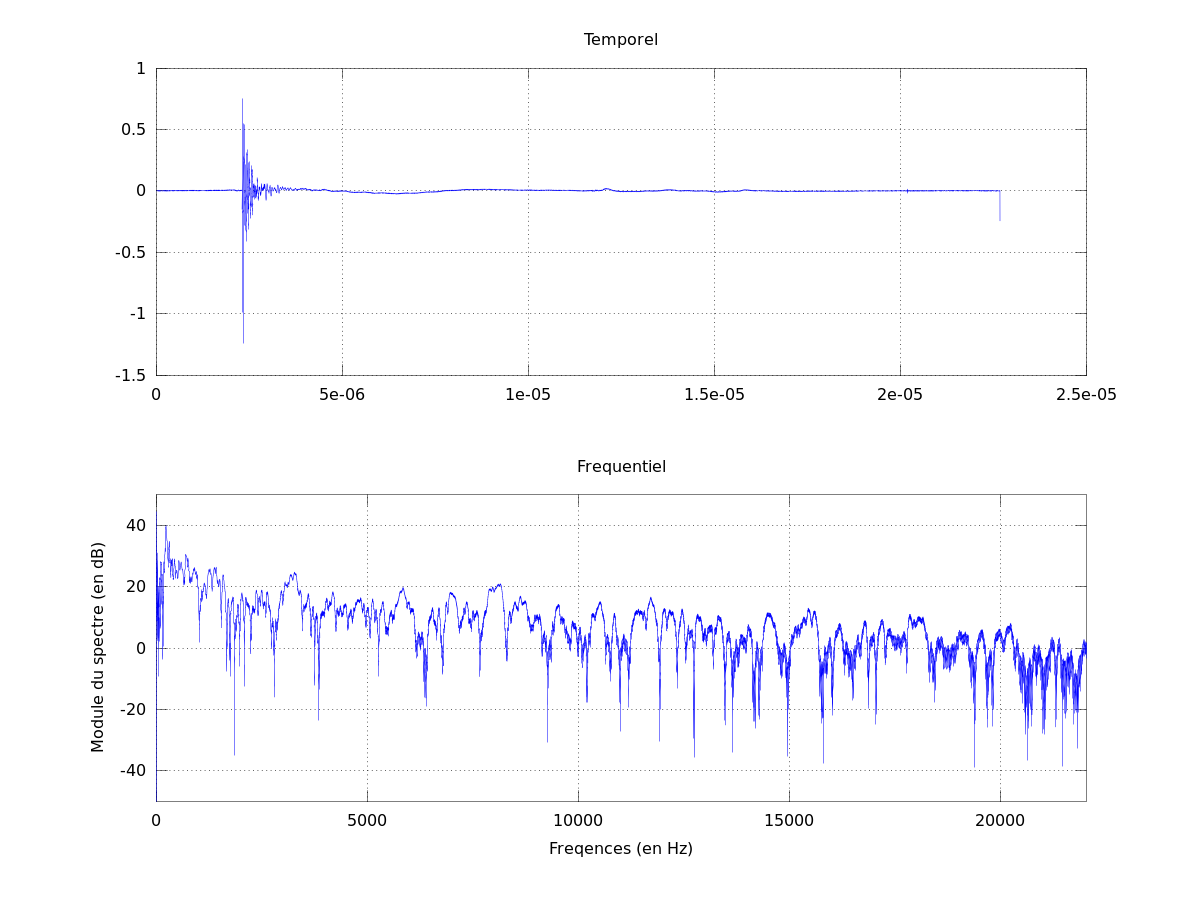
\includegraphics[width=15cm]{rep_ballon_anecho.png}
    \end{center}
    \caption{\label{ballon}Enregistrement temporel et spectre d'un éclatement de ballon de baudruche en salle anéchoïque}
\end{figure}

Pour effectuer la mesure, un microphone est placé au centre de la salle anéchoïque et un ballon de baudruche est éclaté à environ 1m de celui ci. Le manipulateur nécessaire à l'experience est bien sûr  supposé parfaitement absorbant.

Les résultats de la mesure sont disponibles sur le dépot du projet.
Le contenu fréquentiel de l'impulsion créée par le ballon est visible sur la figure~\ref{ballon}.

On constate que le ballon n'a pas une réponse plate en fréquence comme nous l'avions approximé de prime abord. Une grande partie de l'energie se situe dans les basses fréquences (visible par l'amplitude décroissante du spectre du signal).


\section{Objectifs de la séance suivante} % {{{1

Etant donné que nous avons résolu les principaux problèmes rencontrés lors du processus de mesure, la prochaine séance sera entièrement centrée sur l'obtention des données necessaires à la présentation finale du projet. 

Nous allons donc monter une chaîne de mesure mobile et mesurer plusieurs sons anéchoïques dans différentes salles et ce avec et sans la tête permettant une mesure binaurale. Une mesure de ses mêmes sons en salle anéchoïque sera aussi effectuée afin de pouvoir éliminer les eventuelles problèmes de bande passante liés à la chaîne de mesure.

Une fois toutes ces mesures effectuées, nous pourrons comparer percetivement différentes auralisations et voir quels paramètres influent sur le rendu final. 

Une fois ce travail effectué, nous pourrons eventuellement nous interesser à un autre type de source que le ballon tel que le système CLIO par exemple.


\end{document}
